
\section{Interlude: A first look at right triangles} 

\subsection*{Sprinting across the soccer field}

Our university's soccer field measures 117 yards long and 65 yards wide.\footnote{Source: \url{https://athletics.augsburg.edu/sports/2009/3/12/gen031308.aspx?id=5}}  Coach Pelto asked her players to sprint diagonally across the field at practice.  How far is that?

 \begin{center}
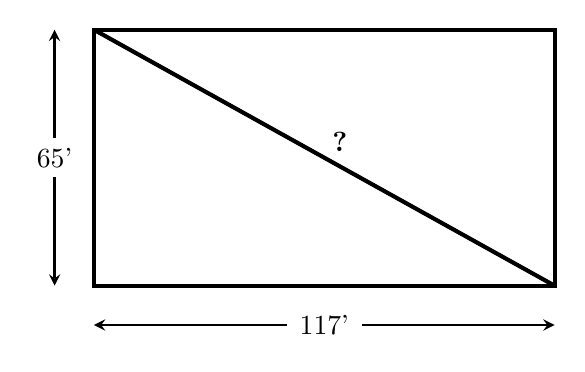
\begin{tikzpicture}[line width=1.5pt, scale = .5]
    % Main Rectangle (S=11.7 units wide + 6.5 units tall)
    \draw (0,0) rectangle (11.7,6.5);
    
    % Bottom Label and arrows
    \draw[<-, >=stealth, line width=0.8pt] (0, -1) -- (4.9, -1);
    \node at (5.85, -1) {117'};
    \draw[->, >=stealth, line width=0.8pt] (6.8, -1) -- (11.7, -1);
    % Left Label and arrows
    \draw[<-, >=stealth, line width=0.8pt] (-1, 0) -- (-1, 2.75);
    \node at (-1, 3.25) {65'};
    \draw[->, >=stealth, line width=0.8pt] (-1, 3.75) -- (-1, 6.5);
    % Diagonal line
    \draw (0,6.5) -- (11.7,0);
    % Diagonal label and arrows
    \node at (6.25, 3.65) {\textbf{?}};
\end{tikzpicture}
 \end{center}

We can say some facts about the diagonal distance.  For one thing, it's definitely longer than length of the longer side which is 117 feet.  Also, sprinting along the edges of the field would be longer than going diagonally, so the diagonal distance is definitely shorter than $65 + 117 = 182$ feet.  So the answer is in between 117 and 182 feet.  I'd guess it's about 150 feet, just because that's a nice number in that range.

\subsection*{The Pythagorean Theorem}

So, how do we find the exact diagonal distance?  Luckily there's a very useful fact called the Pythagorean Theorem.  It says if you have a triangle and if two sides are perpendicular to each other, then there's a formula relating the lengths of the sides. To state the formula we need a little more vocabulary.

The two lines that are perpendicular make an angle of $90^\circ$ which is a \textbf{right angle}.  A triangle that has two sides perpendicular, or equivalently that has a right angle, is cleverly called a \textbf{right triangle}.  The shorter two sides, the ones that are perpendicular are sometimes called the \textbf{legs} of the right triangle.  The longer side, here the diagonal across the field, is called the \textbf{hypotenuse}.  

The \textbf{Pythagorean Theorem} says if you have a right triangle and the legs have length $a$ and $b$ and if the hypotenuse has length $c$, then $$a^2+b^2=c^2$$
(By the way, the opposite is true too: if the equation works, then the two sides are perpendicular.  Carpenters use this fact often to check that they have right angles!)

Back to our problem.  Let's redraw our picture to be a triangle and label width $a=65$ feet, the length $b=117$ feet, and the length of the diagonal $c$ feet.  We mark the angle where the vertical and horizontal meet with a small box to indicate the right angle.  

 \begin{center}
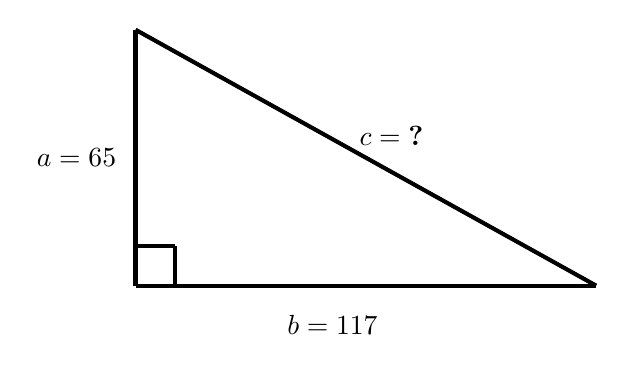
\begin{tikzpicture}[line width=1.5pt, scale = .5]
    % The triangle
    \draw (0,0) -- (0,6.5);
    \draw (0,0) -- (11.7,0);
    \draw (0,6.5) -- (11.7,0);
    % Labels
    \node at (5, -1) {$b=117$};
    \node at (-1.5, 3.25) {$a=65$};
    \node at (6.5, 3.8) {$c=\textbf{?}$};
    % Box indicating perpendicular
    \draw (0,1) -- (1,1);
    \draw (1,0) -- (1,1);
\end{tikzpicture}
 \end{center}

By the Pythagorean Theorem,
$$65^2 + 117^2 = c^2$$
Rewriting to have the variable on the left-hand side of the equation, we get 
$$c^2 = 65^2 + 117^2 = 17914$$
We can use square roots to find $c$,
$c = \sqrt{17914} = 133.8431\ldots \approx 133.8 \textbf{ feet}$
Our estimate of 150 feet was a bit high, but pretty close!

\subsection*{Hanging a wall banner}

After practice, Coach Pelto asked Marta to help put up a banner on the side wall.  Marta was able to find a 16 foot ladder.  She placed the base of the ladder 4 feet away from the wall and let the ladder lean against the wall. How high up on the wall was the top of the ladder?

Let's start by drawing a picture.  It doesn't matter which leg of the triangle we label $a$ and which we label $b$.  But it does matter that $c$ is the hypotenuse, the longest side, the side opposite the right angle.

 \begin{center}
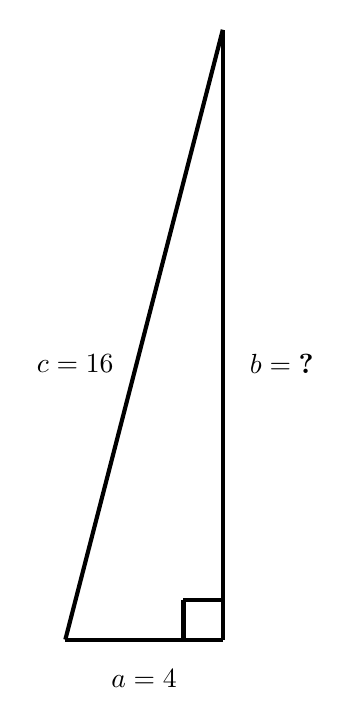
\begin{tikzpicture}[line width=1.5pt, scale = .5]
    % The triangle
    \draw (0,0) -- (4,0);
    \draw (4,0) -- (4,15.491);
    \draw (0,0) -- (4,15.491);
    % Labels
    \node at (2, -1) {$a=4$};
    \node at (0.25, 7) {$c=16$};
    \node at (5.5, 7) {$b=\textbf{?}$};
    % Box indicating perpendicular
    \draw (3,1) -- (4,1);
    \draw (3,0) -- (3,1);
\end{tikzpicture}
 \end{center}
We can use the Pythagorean Theorem to get the equation
$$4^2+b^2=16^2$$
Evaluating the squares we get
$$16+b^2 = 256$$
Subtracting 16 from each side we get
$$b^2=240$$
Then
$$b=\sqrt{240} =15.4919\ldots \approx 15.5 \text{ feet}$$
The top of the latter will be about 15'6" high.  Luckily Marta is brave and climbs the ladder to hang the banner.

\subsection*{Why is the Pythagorean Theorem true?}

In case you're curious, there's a lovely proof by picture\footnote{For a discussion of the origins of this proof, and many more, see \url{https://www.cut-the-knot.org/pythagoras/}} that shows that the Pythagorean Theorem is true.  In the picture, the red squares have area $a^2$ and $b^2$, the big blue square has area $c^2$, each of the four yellow right triangles has sides of length $a$, $b$, and $c$, and the outer squares are the same dimension: $(a+b) \times (a+b)$.  Since the outer squares have the same area and the four yellow triangles have the same area, the red area ($a^2+b^2$) must be the same as the blue area ($c^2$).  Woo hoo!

\begin{center}
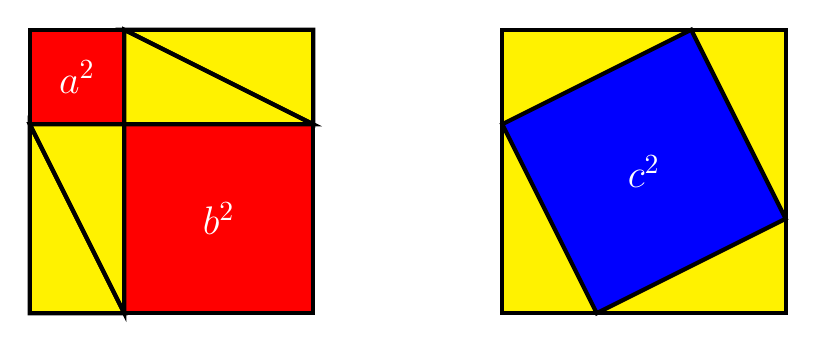
\begin{tikzpicture}[scale=0.6, line width=1.5pt]
  \def\a{2}
  \def\b{4}
  \def\s{6} % s = a + b = 6

  % ================= LEFT FIGURE (a^2 + b^2) =================
  \begin{scope}[shift={(0,0)}]
    % Four Triangles (Yellow)
    \fill[yellow] (0,0) -- (\a,0) -- (0,\b) -- cycle;
    \fill[yellow] (\a,\s) -- (\s,\s) -- (\s,\b) -- cycle;
    \fill[yellow] (\a,\b) -- (\s,\b) -- (\a,\s) -- cycle;
    \fill[yellow] (0,\b) -- (\a,\b) -- (\a,0) -- cycle;

    % Two Inner Squares (Red)
    % Small Square (a^2) at Top-Left
    \fill[red] (0,\b) rectangle (\a,\s);
    \node at (\a/2, \b + \a/2) [color=white] {\Large $a^2$};
    
    % Large Square (b^2) at Bottom-Right
    \fill[red] (\a,0) rectangle (\s,\b);
    \node at (\a + \b/2, \b/2) [color=white] {\Large $b^2$};

    % Internal Lines & Outer Border
    \draw (0,0) -- (\a,0) -- (0,\b) -- cycle;
    \draw (\a,\s) -- (\s,\s) -- (\s,\b) -- cycle;
    \draw (\a,\b) -- (\s,\b) -- (\a,\s) -- cycle;
    \draw (0,\b) -- (\a,\b) -- (\a,0) -- cycle;
    
    \draw (0,0) rectangle (\s,\s);
    \draw (0,\b) -- (\s,\b);
    \draw (\a,0) -- (\a,\s);
  \end{scope}

    % ================= RIGHT FIGURE (c^2) =================
  \begin{scope}[shift={(10,0)}]
    % Outer Square / Four Triangles
    \fill[yellow] (0,0) rectangle (\s,\s);
    
    % Inner Rotated Square (c^2)
    \fill[blue] (\a,0) -- (\s,\a) -- (\b,\s) -- (0,\b) -- cycle;
    \draw (\a,0) -- (\s,\a) -- (\b,\s) -- (0,\b) -- cycle;
    
    % Outer Border
    \draw (0,0) rectangle (\s,\s);
    
    % Inner Label
    \node at (\s/2, \s/2) [color=white] {\Large $c^2$};
  \end{scope}
\end{tikzpicture}
\end{center}

 \input{GoDoWS}

\noindent \textbf{Do you know \ldots}

\begin{itemize}
\item What a right angle and a right triangle are?
\item What the short sides and the longest side of a right triangle are called?
\item How to use the Pythagorean Theorem to find the length of a side of a right triangle?
\item When to use the Pythagorean Theorem?
 \input{NotSure} 
\end{itemize}

\subsection*{Exercises}

\begin{enumerate} 
%% WORKBOOK

\item Beau and Kurt are warming up before their ultimate frisbee match in a parking lot which is $289' \times 122'$.  They stand at diagonal corners to throw the frisbee.  How far apart at they?
\begin{enumerate}
    \item Draw a picture of a right triangle that illustrates the information from the story.
    \item Estimate the answer.  Hint: Explain why it's gonna be greater than 289' and less than 411'.
    \item Which sides of the triangle do we know the length of and which side are we looking for the length of?  Label them $a$, $b$, and $c$.  Measure the lengths in feet.
    \item What equation does the Pythagorean Theorem give you?
    \item Solve that equation to answer the question. %Answer 313.6
\end{enumerate}

\item As part of an environmental engineering lab, your group is installing a solar panel on a flat campus roof. The solar panel needs to be mounted at an angle. The panel itself is 6'6" wide with one edge sitting essentially on the roof and the opposite edge elevated 24" above the roof.  What is the horizontal width of the ``footprint'' area below the solar panel on the roof. (That would matter, for example, if we were trying to fit more solar panels up there.)

\begin{enumerate}
    \item Draw a picture of a right triangle that illustrates the information from the story.
    \item Let's measure the lengths in inches, so you need to convert 6'6" to inches.
    \item Which sides of the triangle do we know the length of and which side are we looking for the length of?  Label them $a$, $b$, and $c$.  
    \item What equation does the Pythagorean Theorem give you?
    \item Solve that equation to answer the question.
\end{enumerate}

\item Satoshi is setting up his apartment.  He wants to work on his laptop at his standing desk which is 43" tall. Satoshi stands at the side of the desk closest to the nearby wall outlet (and right in front of the outlet).  He wants to plug his computer charger into the top plug which is 14" above the floor. Satoshi's laptop sits  a comfortable distance away on the desk top.  He measures that it's 9" from the edge of the desk to the charger port. 

If Satoshi's places his desk is 36" from the wall, will he be able to plug in his laptop using a 4-foot long cord?  As part of your work, draw a right triangle, label the sides, use the Pythagorean Theorem to set up an equation, and solve to determine how long the cord needs to be.  Be sure to answer the question at the end. Hint: Notice that the charger port is $36+9 = 45"$ from the wall.  Also notice that the and the charger port and outlet plug are $43-14 = 29"$ apart in height. % Answer a = 29, b = 45, so c = 53.5"  Nope.

\item Nope, that 4-foot long cord isn't long enough for Satoshi to charge his laptop.  He's gonna have to move the desk closer to the wall.  How close to the wall does Satoshi need move the desk so he can charge his laptop while he works?  As part of your work, draw a right triangle, label the sides, use the Pythagorean Theorem to set up an equation, and solve to determine how far away from the wall his desk can be.  At the end, subtract 9" to find the distance from his desk to the wall. Hint: Don't forget to convert 4 feet to inches. % Answer a = 29, c = 48, so b = 38.2"  subtract 9" to get 29.2".  The table can be about 29" from the wall 

%% HOMEWORK 

\item Central Park in New York City is 2.5 miles long (from 59th Street in Midtown to 110th Street in Harlem) and 1 mile wide (from Fifth Avenue to Eighth Avenue).\footnote{Source: \url{https://en.wikipedia.org/wiki/Central_Park}} It's impossible to walk exactly diagonally across the park because of The Lake and the reservoir, but if you could, how far would that be?
\begin{enumerate}
    \item Explain why the answer is more than 2.5 miles and less than 3.5 miles.  What's a good guess for the answer?
    \item Draw a picture of a right triangle that illustrates the information from the story.
    \item Which sides of the triangle do we know the names of and which side are we looking for?  Label them $a$, $b$, and $c$.  Measure the lengths in miles.
    \item What equation does the Pythagorean Theorem give you?
    \item Solve that equation to answer the question.
\end{enumerate}

\item Judith is having an accessible ramp built on the women's health clinic where she volunteers.  The entrance to the building is 4 feet above the ground which is otherwise flat.  Guidelines under the ADA\footnote{The Americans with Disabilities Act \url{https://en.wikipedia.org/wiki/Americans_with_Disabilities_Act_of_1990}} require 12 inches of ramp length for every 1 inch of rise.
\begin{enumerate}
    \item To get 4 feet of rise, how long will the ramp need to be?
    \item Draw a right triangle illustrating the situation and label the known and unknown side lengths.
    \item Assuming the ramp is straight, how far away from the building does the ramp need to start?  (In practice, ramps often zig-zag back and forth to fit in the available space.)
\end{enumerate}

\item Marine biologists tracking a humpback whale attach an electronic tag that transmits acoustic pings to a research boat. The direct distance from the boat to the submerged whale is 203 meters. The boat's GPS shows it is located 194 meters horizontally along the water's surface from the point directly above the whale.  How deep under the water's surface is the whale?  As part of your work, draw a right triangle, label the lengths of the sides, and use the Pythagorean Theorem.  Hint:  humpback whales frequently dive around 80 meters deep.\footnote{Source: \url{https://en.wikipedia.org/wiki/Humpback_whale}}

\item Bob is building a roof truss, as shown in the picture, for the new backyard shed he's building.  The King Post is vertical and will be 5 feet tall.  The Tie Beam is horizontal and will be 24 feet long.  Note that the King Post lands exactly in the middle of the Tie Beam.


\begin{center}
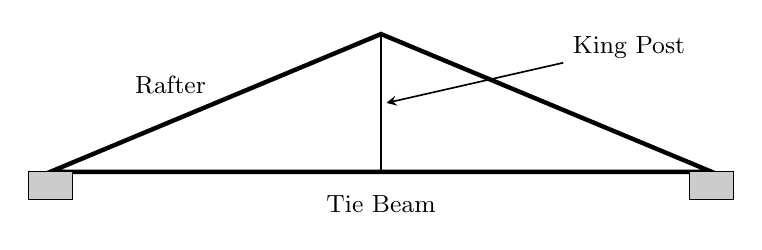
\begin{tikzpicture}[scale=0.35]
    % Coordinates for the King Post Truss
    \coordinate (A) at (0,0);       % Left support
    \coordinate (B) at (24,0);      % Right support
    \coordinate (C) at (12,5);      % Peak (Apex)
    \coordinate (M) at (12,0);      % Midpoint on bottom chord

    % Main Outer Frame (Chords)
    \draw[ultra thick] (A) -- (B) -- (C) -- cycle;

    % Vertical Central Support (King Post)
    \draw[thick] (C) -- (M);

    % Ground Support Blocks
    \draw[fill=gray!40] (-0.8,-1) rectangle (0.8,0);
    \draw[fill=gray!40] (23.2,-1) rectangle (24.8,0);

    % Component Labels
    \node[above left] at (6, 2.5) {\small Rafter};
    \node[below] at (12, -0.5) {\small Tie Beam};

    % King Post Label positioned safely to the right of the rafter
    \node (kp) at (21, 4.5) {\small King Post};
    \draw[->, >=stealth, semithick] (kp) -- (12.2, 2.5);
\end{tikzpicture}
\end{center}

\begin{enumerate}
    \item Draw a right triangle showing just the left-hand side of the roof and label the sides of your triangle with the information given in the story, or a letter if we don't know the length.
    \item Use the Pythagoream Theorem to find the length of the rafter.
    \item Did anything about the length surprise you?
\end{enumerate}

\item Use the Pythagoream Theorem  to confirm that each of the following triples could be the lengths of a right triangle. 
\begin{enumerate}
    \item 3 yards, 4 yards, 5 yards
    \item 5 feet, 12 feet, 13 feet
    \item 8 cm, 15 cm, 17 cm
    \item 7 miles, 24 miles, 25 miles
\end{enumerate}

\end{enumerate}

\bigskip

\noindent \textbf{When you're done \ldots}

\begin{itemize}
\item Don't forget to check your answers with those in the back of the textbook. 
\item Not sure if your answers are close enough? Compare with a classmate or ask the instructor.  
\item Getting the wrong answers or stuck on a problem?  Re-read the section and try the problem again.  If you're still stuck, work with a classmate or go to your instructor's office hours.
\item It's normal to find some parts of some problems difficult, but if all the problems are giving you grief, be sure to talk with your instructor or advisor about it.  They might be able to suggest strategies or support services that can help you succeed.
\item Make a list of key ideas or processes to remember from the section.  The ``Do you know?'' questions can be a good starting point.
\end{itemize}



